 % !TEX TS-program = pdflatex
% !TEX encoding = UTF-8 Unicode



\documentclass[slidetop,11pt]{beamer}

\usepackage[francais]{babel}
\usepackage[T1]{fontenc}
\usepackage[utf8]{inputenc}

\usepackage{amsmath,amsfonts,amssymb,ulem,epigraph}

\usepackage[upright]{fourier}

\usepackage{shadethm}

\usepackage{subfig}

\usepackage{pgf,tikz}
\usetikzlibrary{arrows}

\usepackage{color}
\definecolor{gris_clair}{gray}{.9}
\definecolor{gris}{gray}{.35}
\definecolor{vert}{rgb}{0,0.5,0}
\definecolor{rouge}{rgb}{0.5,0,0}
\definecolor{turquoise}{rgb}{0,0.5,0.5}

%\graphicspath{{./} {./experience/utiliteordrecontrainte/}}

\usepackage{listings}           
\lstset{
language=Caml,
backgroundcolor=\color{gris_clair},
frame=single,
basicstyle=\footnotesize\ttfamily\color{gris},
identifierstyle=\color{black},
keywordstyle=\color{vert},
stringstyle=\color{rouge}, showstringspaces=false,
commentstyle=\itshape\color{turquoise},
%numbers=left, numbersep=5pt, numberstyle=\color{gris}\tiny,stepnumber=5,
breaklines=true,
literate=
  {é}{{\'e}}1 {É}{{\'E}}1 {à}{{\`a}}1 {è}{{\`e}}1% 
  {À}{{\`A}}1 {È}{{\'E}}1 {ë}{{\"e}}1 {ï}{{\"i}}1%
  {â}{{\^a}}1 {ê}{{\^e}}1 {î}{{\^i}}1 {ô}{{\^o}}1% 
  {û}{{\^u}}1 {Â}{{\^A}}1 {Ê}{{\^E}}1 {Î}{{\^I}}1%
  {Ô}{{\^O}}1 {œ}{{\oe}}1 {Œ}{{\OE}}1 {æ}{{\ae}}1%
  {Æ}{{\AE}}1 {ç}{{\c c}}1 {Ç}{{\c C}}1 {€}{{\EUR}}1 ,
morekeywords={len,input,range}}

\usetheme{Warsaw}
\usecolortheme{beaver}

\graphicspath{{./} {./../source/}}

\title{Autour du Manège Enchanté}
\subtitle{intersections routières}
\date{}
\author{Antonin Dudermel}

\begin{document}

\newshadetheorem{defin}{Définition}
\newshadetheorem{theo}{Théorème}

\frame{\titlepage}

\begin{frame}
	\epigraph{Tournicoti, tournicotin}{\it Zébulon}
\end{frame}

\begin{frame}
	\tableofcontents
\end{frame}

\section{Modéliser un rond-point}

	\subsection{Un Automate cellulaire}
		\begin{frame}
	\frametitle{Modèle Nagel-Schreckenberg (NaSch)}
	\begin{enumerate}
		\item Accélération 
		\item Décélération
		\item Facteur aléatoire
		\item Mouvement
	\end{enumerate}
\end{frame}

\begin{frame}
Accélération
	Avec $v_i$ la vitesse de la voiture $i$, $v_{max}$ la vitesse maximale autorisée : 
	\begin{equation}
		v_i \leftarrow \min (v_i+1,v_{max})
	\end{equation}
\\

Décélération
	avec $d_i$ la distance entre les voitures $i$ et $i+1$
	\begin{equation}
		v_i \leftarrow \min (v_i,d_i-1)
	\end{equation}


Facteur aléatoire
	\begin{equation}
		v_i \leftarrow \max(v_i-1,0) \text{ avec proba } p
	\end{equation}
	Mouvement
	\begin{equation}
		x_i \leftarrow x_i + v_i
	\end{equation}
\end{frame}


\begin{frame}
\frametitle{validité}
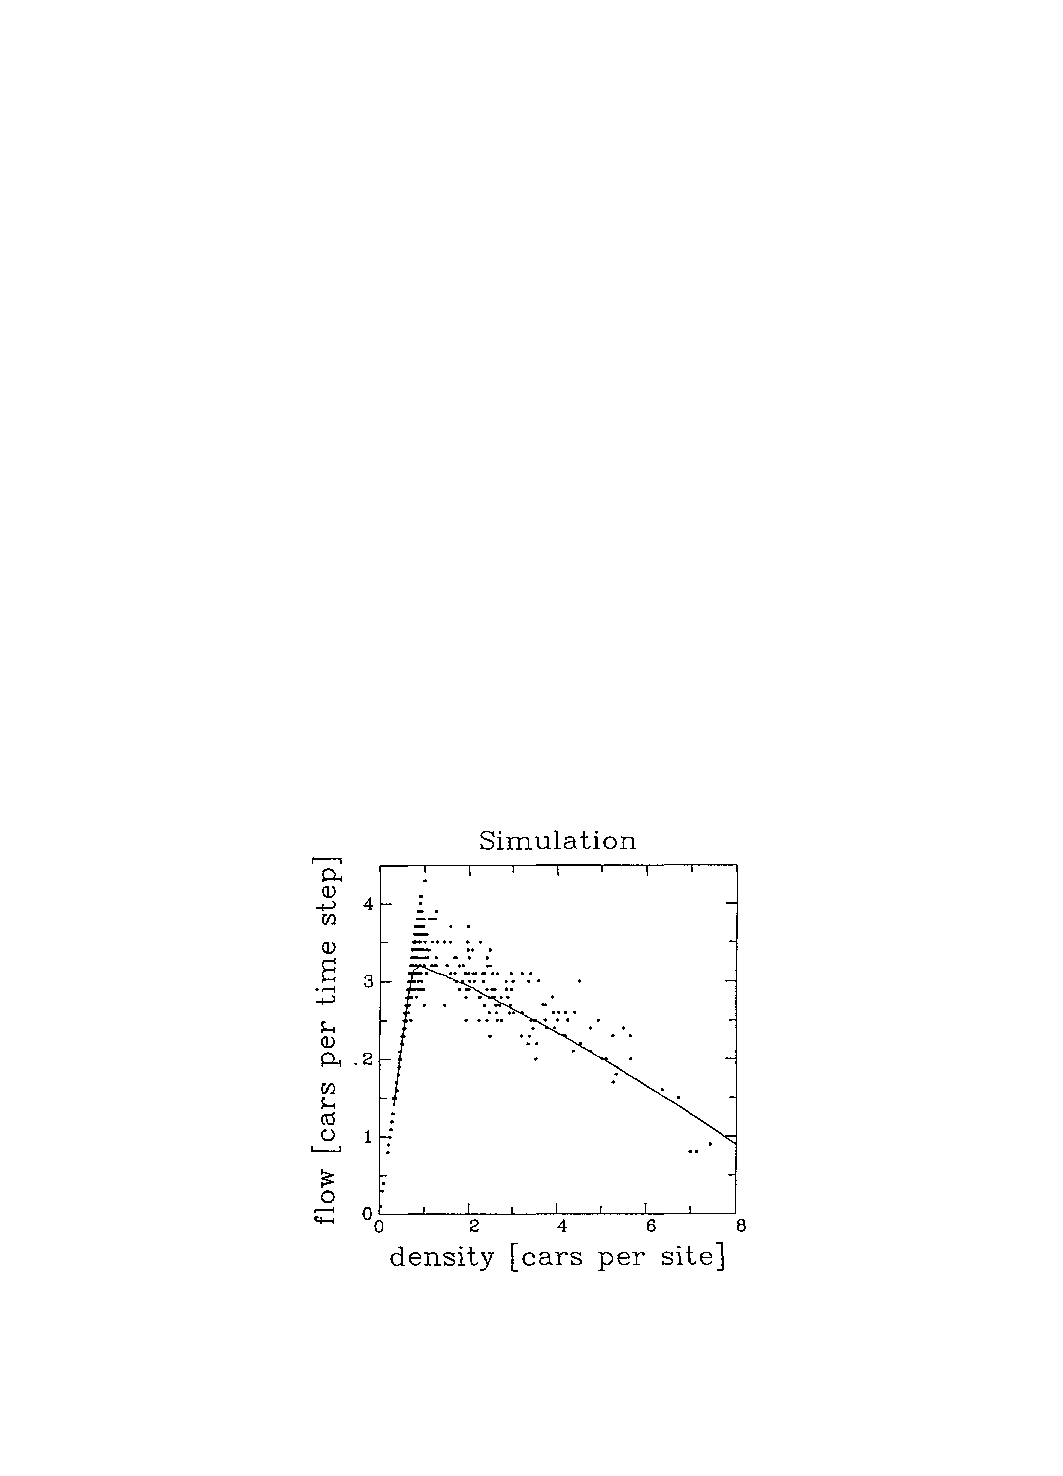
\includegraphics[scale = 0.7]{./images/dfondcomp}
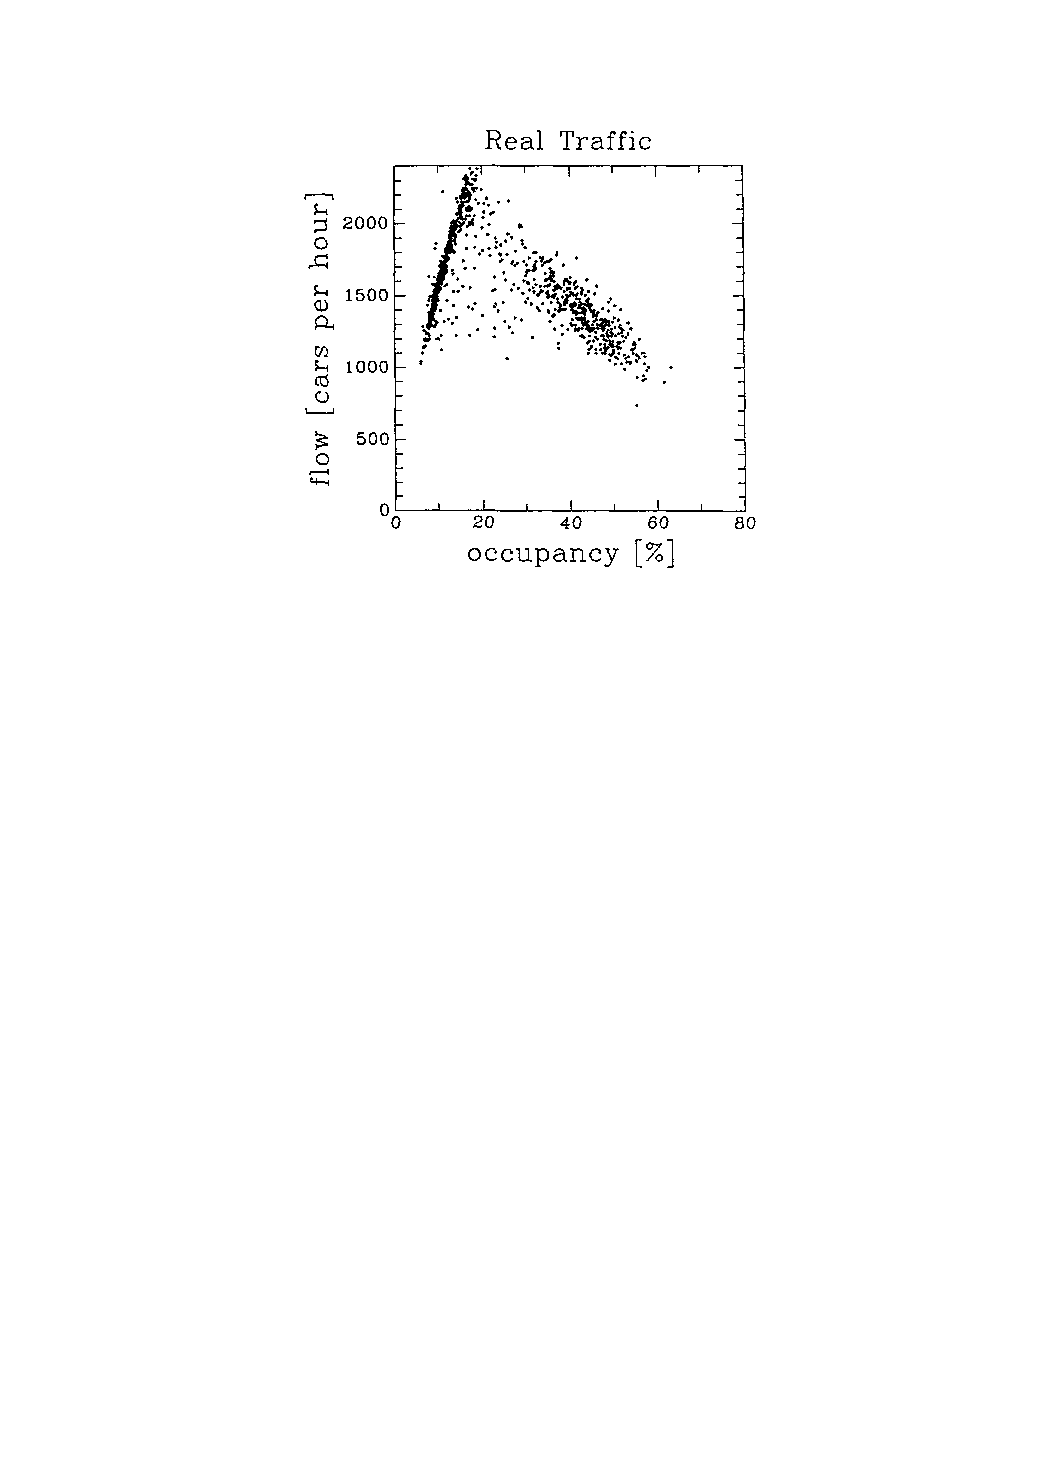
\includegraphics[scale = 0.7]{./images/dfondcompre}
\end{frame}

	\subsection{Le problème des intersections}
\begin{frame}
\frametitle{adapter le modèle}
	Deux types d'objets : les sections et les intersections. Il faut déterminer les comportements aux intersections
\end{frame}	

\begin{frame}
	\frametitle{un premier modèle : priorité absolue}
	\begin{figure}
		\begin{center}
			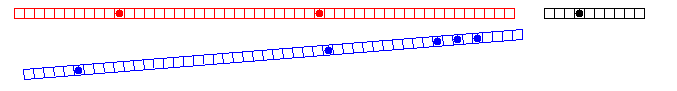
\includegraphics[scale=0.5]{./images/localdebut}
		\end{center}
		\caption{Un exemple d'intersection 2-1}
	\end{figure}
	
	Si une voiture de la voie prioritaire décide de passer, la voiture non-prioritaire la laisse passer : on indente la première mais pas la deuxième.
\end{frame}	
	
	
\begin{frame}
	\frametitle{Modèle Rui-Xiong, Ke-Zhao, Liu Mu-Ren}
	Idée : anticiper le mouvement des deux voitures souhaitant passer, puis indenter les voitures l'une après l'autre
		\begin{equation}
			t_i = \frac{x_I - x_i}{\min(v_{max},d_i-1,v_i+1)}
		\end{equation}
\end{frame}
	\subsection{Étude locale : comparer les modèles sur une intersection}

\begin{frame}
	\frametitle{Étude locale}
	Expérience simpliste : deux entrées et une sortie \\
	Objectifs
	\begin{enumerate}
		\item Chercher les limites du modèle
	 	\item Chercher les limites du rond-point
		\item Déterminer les différences entre les deux modèles
	\end{enumerate}
	\begin{figure}
		\begin{center}
			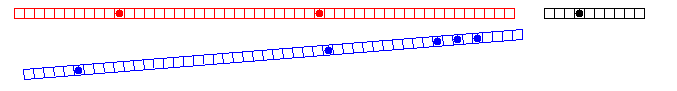
\includegraphics[scale=0.5]{./images/localdebut}	
		\end{center}
		\caption{L'expérience en cours}
	\end{figure}		
\end{frame}	

\begin{frame}
	\frametitle{Méthode d'étude : le diagramme fondamental}
	Grandeurs étudiées : 
	\begin{itemize}
		\item flux $J \text{ en } \mathrm{veh}/\mathrm{s}$
		\item vitesse $v \text{ en } \mathrm{m}/\mathrm{s}$
		\item densité $\rho \text{ en } \mathrm{veh}/\mathrm{m}$
	\end{itemize}
	$$J = \rho<v>$$
\end{frame}

\begin{frame}
	\frametitle{Diagramme fondamental}
	$$J = f(\rho)$$
	\begin{figure}
		\begin{center}	
			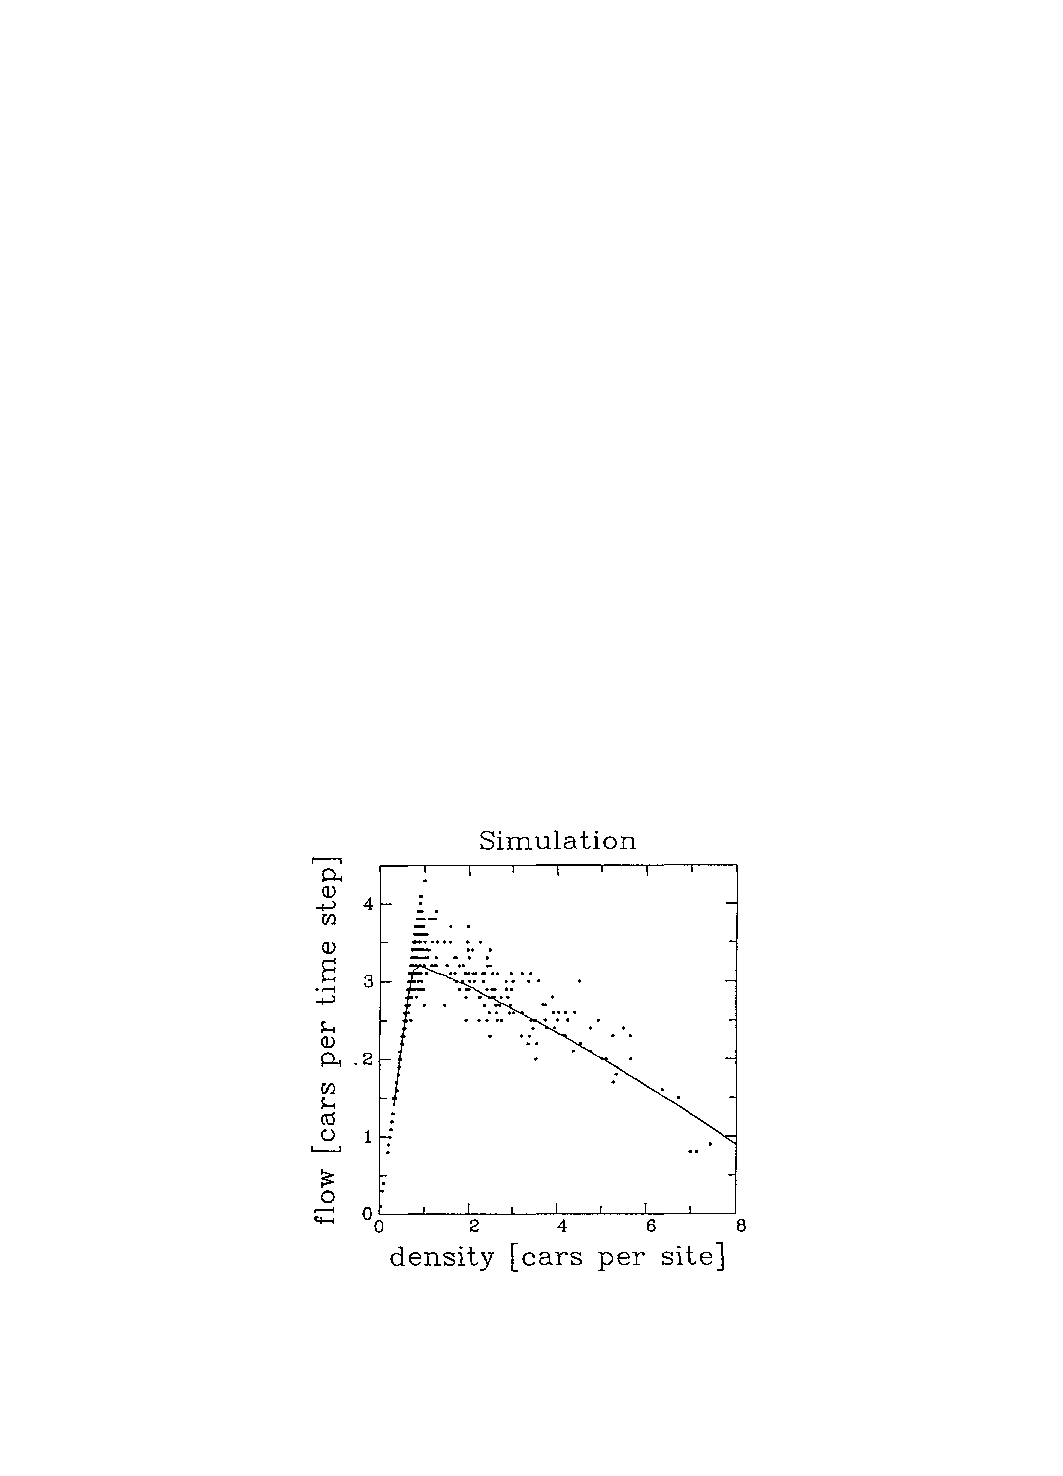
\includegraphics[scale = 0.7]{./images/dfondcomp}
		\end{center}
	\caption{Un exemple de diagramme fondamental}
	\end{figure}
\end{frame}
	
\begin{frame}
	\frametitle{Expérience :}
	Sur la voie non-prioritaire : un flot continu et peu dense de voitures.\\
	Sur la voie prioritaire : un flot croissant de voitures.
\end{frame}
	
\begin{frame}
	\frametitle{Premiers résultats}
	\begin{figure}
		\begin{center}
			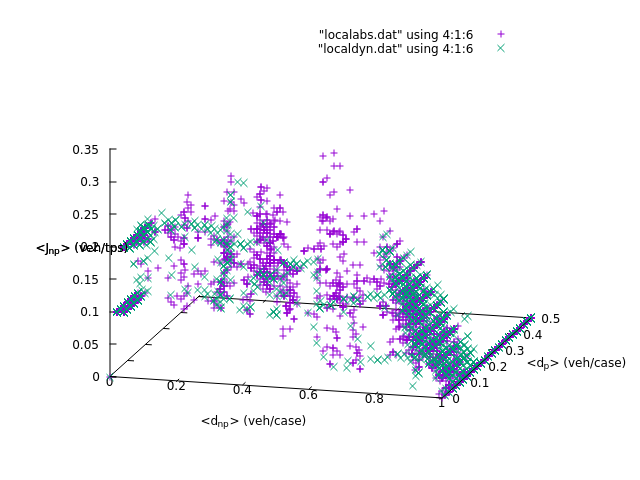
\includegraphics[scale=0.4]{./diagrammes-fondamentaux/localabsdyn0w}
		\end{center}
	\caption{Comparaison absolu-dynamique}
	\end{figure}
\end{frame}

\begin{frame}
	\frametitle{Interprétation}
	Informations : 
		\begin{itemize}
			\item Met en évidence le problème de ces intersections
			\item On ne voit pas une grande différence entre les deux modèles		
		\end{itemize}
		
	Améliorations possibles :
		\begin{itemize}
			\item Étudier un champ plus réduit
			\item Modifier le modèle
		\end{itemize}

\end{frame}

\begin{frame}
	\frametitle{Champ réduit}
		\begin{figure}
		\begin{center}
			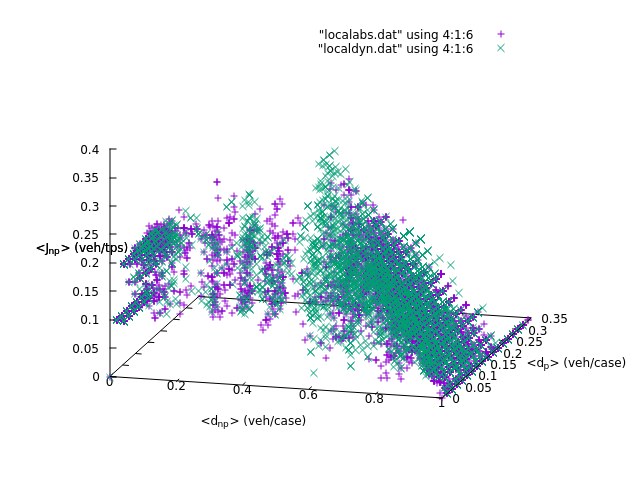
\includegraphics[scale=0.4]{./diagrammes-fondamentaux/localabsdyn0wred}
		\end{center}
	\caption{Comparaison sur un champ réduit}
	\end{figure}
\end{frame}

\begin{frame}
	 \frametitle{Améliorer le modèle}
	 Ajout d'un temps de réaction pour un redémarrage.
	 \begin{figure}
	 	\begin{center}
	 		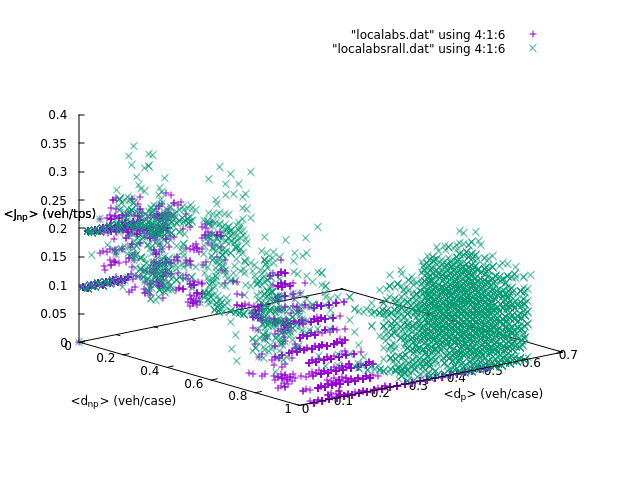
\includegraphics[scale=0.4]{./diagrammes-fondamentaux/localabs0w1w}
	 	\end{center}
	 	\caption{Étude locale avec temps de démarrage}
	 \end{figure}
\end{frame}

\begin{frame}
	\frametitle{Résultats}
	Observations :
		\begin{itemize}
			 \item Blocage à des densités plus élevées
			 \item Une différence entre les modèles
		\end{itemize}
	Explications :
		\begin{itemize}
			\item saturation de la voie principale
			\item augmentation de l'importance de l’arrêt
		\end{itemize}
	\begin{figure}
		\begin{center}
			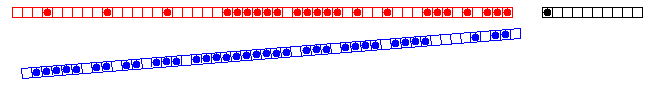
\includegraphics[scale=0.4]{./images/localsature}
		\end{center}
		\caption{début de saturation}
	\end{figure}
\end{frame}

\begin{frame}
	\frametitle{Comparaison}
	\begin{figure}
		\begin{center}
			\subfloat[temps 1]{
				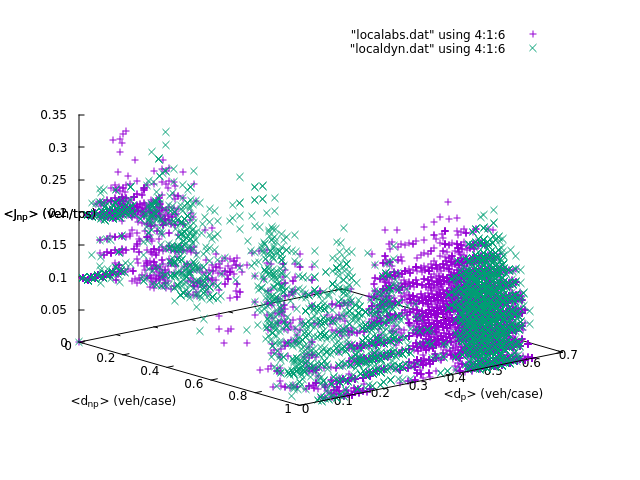
\includegraphics[scale=0.35]{./diagrammes-fondamentaux/localabsdyn1w}
			}
			\subfloat[temps 2]{
				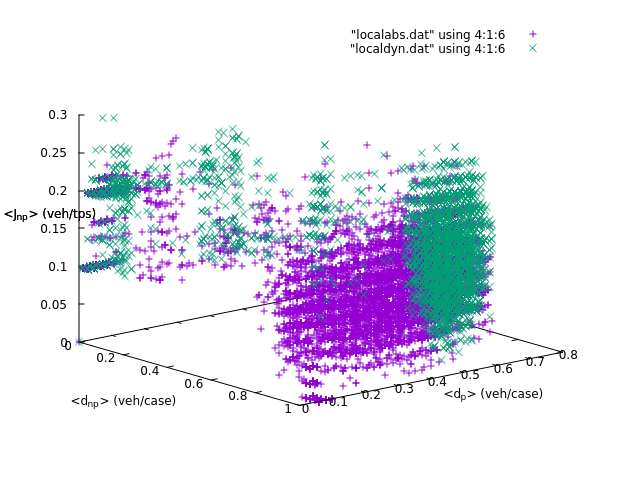
\includegraphics[scale=0.35]{./diagrammes-fondamentaux/localabsdyn2w}
			}
		\end{center}
	\end{figure}
\end{frame}
\section{Études sur des ronds-points}
	\subsection{expériences prévues}

\begin{frame}
	\frametitle{Rond-point et feux de croisement}
	tests pour :
	\begin{itemize}
		\item autant de voitures de chaque coté
		\item plus de voitures d'un coté
		\item plus de voitures avec feux adaptés
		\item feux mal adaptés
	\end{itemize}
	
	\frametitle{Différents ronds-points}
	Objectif : déterminer l'influence de la circonférence du rond-point (test sur des circonférences différentes \\
	Problème : géométries très différentes : peut-être étudier des données propres à chaque voiture comme le temps passé dans le rond-point
\end{frame}

	
\section{Le Manège enchanté}
	\subsection{Le Manège}
\begin{frame}
	\begin{center}
		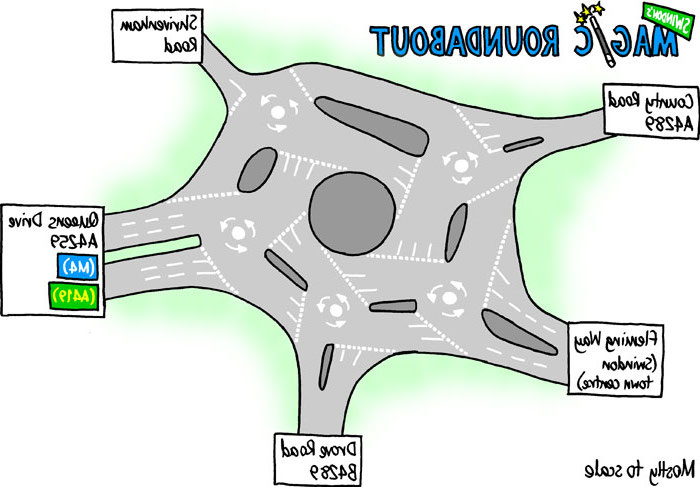
\includegraphics[scale=0.4]{./images/magic}
	\end{center}
\end{frame}

\begin{frame}
	\frametitle{Fonctionnement}
	\begin{itemize}
		\item 1 grand rond-point central tournant dans le sens inverse
		\item 5 petits ronds-points latéraux
		\item Des lignes de "cédez le passage" avec de l'espace pour plusieurs voitures
	\end{itemize}
\end{frame}

\begin{frame}
	\frametitle{Comment circuler ?}
	\begin{figure}
		\begin{center}
			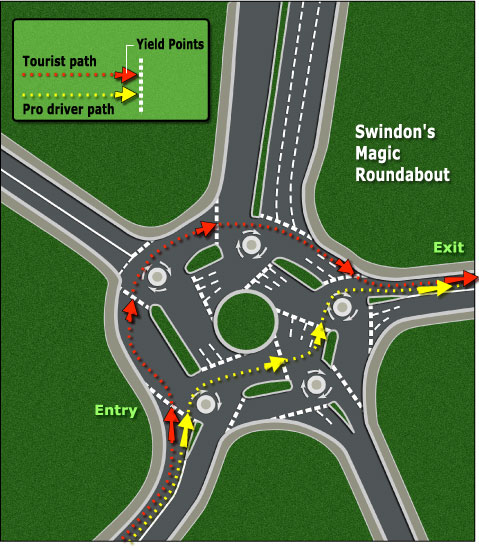
\includegraphics[scale=0.3]{./images/itin}
			\caption{itinéraires possibles}
		\end{center}
	\end{figure}
\end{frame}

	\subsection{Limites du modèle pour le manège}
	
\begin{frame}
	\frametitle{Difficultés à modéliser}
	\begin{itemize}
		\item de nombreux objets
		\item routes de tailles variables : besoin de connaître les fréquences de chaque route
		\item le modèle ne tient pas compte des multiples entrées
	\end{itemize}
\end{frame}
	\subsection{Une Étude avec la théorie des graphes}

\begin{frame}
	\frametitle{Graphe du rond-point}
	\begin{figure}
		\begin{center}
			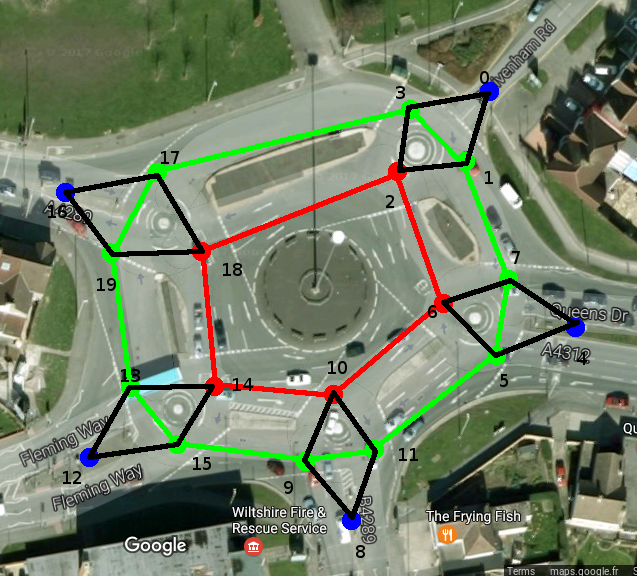
\includegraphics[scale=0.3]{../manege-graphe}
		\end{center}
		\caption{le graphe du manège}
	\end{figure}
\end{frame}

\begin{frame}
	\frametitle{chemins plus courts}
	Objectif : appliquer Floyd-Warshall pour montrer une diminution du trajet
\end{frame}

\begin{frame}
	\frametitle{résistant aux accidents ?}
	Supposons qu'il y ait un accident sur une section, le rond-point est-il toujours fonctionnel ?
\end{frame}

\begin{frame}
	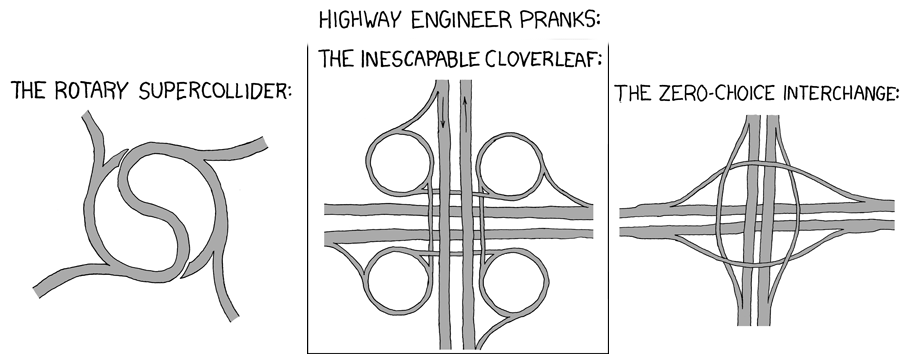
\includegraphics[scale=3]{./images/highway-engineers-pranks-hz}
\end{frame}

\end{document}